\chapter{Софтуерна реализация}
\label{chap:software}
% TODO: ask Garistov if 1/4 sec is enough for magic smoke to appear
% TODO: ask Garistov what to do with the messed up interupts
Използваната среда за разработка на софтуерната част от дипломния проект е софтуерния пакет STM32CubbeIDE на STMicroelectronics. Тази платформа е предназначена за изграждане на софтуерното управление на STM микроконтролери и микропроцесори. Чрез интеграцията на GNU GCC компилатор и GBD дебъгер, тя предоставя стабилна среда за разработка на C/C++ програми. В STM32CubbeIDE е интегриран и графичния инструмент STM32CubeMX. Той улеснява конфигурацията и инициализацията на различни части и периферии на микроконтролерите, сред които са пинове, таймери, системни прекъсвания и DMA заявки. Друга основна характеристика на избраната среда за разработка е възможността за подробен дебъгване чрез мониторинг на процесорните ядра, регистрите на периферията, паметта и заделените променливи и други. Софтуерният пакет може да бъде свален безплатно от сайта на STMicroelectronics за 64-битовите версии на операционните системи Windows, Linux и macOS. Поради споменатите причини тази среда за разработка беше използвана за проекта.


%================================================================================
% ЛОГИЧЕСКА СХЕМА  -  РОБОТ

\section{Логическа схема на проекта}
\label{sec:logic-schemas}

Съгласно заданието на дипломния проект разработеният боен робот бива управляван посредством специално изработено дистанционно. Комуникацията между тях бива реализирана посредством радиочестотните модули nRF24L01 на компанията Nordic. Те използват вградения си протокол за комуникация Enhanced ShockBurst, който е предназначен за лесна комуникация с ниска енергийна консумация.

Като се получи захранване микроконтролера и радиочестотния модул в дистанционното биват инициализирани. След това започва непрекъснато повтарящият се на равни интерваи цикъл на работа. Първо се прочитат входните данни от потенциометрите и бутоните. След това те биват обработени и записани в подходящ вид. В края на този цикъл обработените потребителски команди биват записани в пакет с инструкции за контрол на бойния робот и той бива изпратен към батълбота за изпълнение. После цикъла на работа на дистанционното започва да се изпълнява отначало. Микроконтролерът е настроен да може да бъдат изпращани по 20 пакета с команди в секунда. Това скорост гарантира на пилота възможността да може да управлява своята машина с минимално системно забавяне.

\begin{figure}[H]
    \centering
    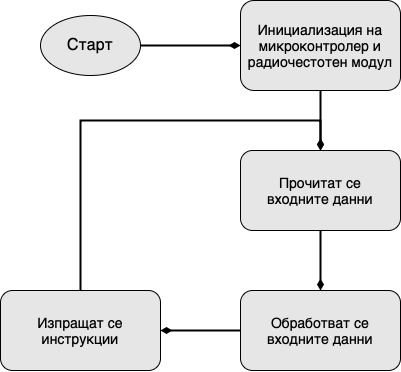
\includegraphics[width=0.6\linewidth]{images/logic-schema-controller.png}
    
    \caption{Логическа схема на дистанционното}
    \label{fig:logic-controller} 
\end{figure}

Полетата, които се съдържат в изпратения пакет са инструкция за позицията, на която трябва да застане механичната ръка на робота, инструкции за скоростта и посоката на въртене на двете колела и инструкция за това дали оръжието трябва да се върти. Структурата на такъв пакет може да бъде видяна на \autoref{lst:payload}.

\lstinputlisting[language=c, consecutivenumbers=false, linerange={11-17}, caption={Пакет инструкции}, label={lst:payload}]{documents/rf-library/NRF24L01.h}

Подобно на дистанционното първата работа на печатната платка, когато получи захранване е да се инициализират микроконтролера и радиочестотния модул. След това започва непрекъснат цикъл на проверяване дали има получен пакет инструкции и ако има се прави опит той да бъде достъпен. При успешното им прочитане те биват заредени в паметта на платката и биват изпълнени. След тази стъпка следва повторно започване на работния цикъл на робота. В случаите, в които няма получени инструкции или не бъде успешно тяхното прочитане, цикъла на работа започва отначало и се спира движението на робота.

\begin{figure}[H]
    \centering
    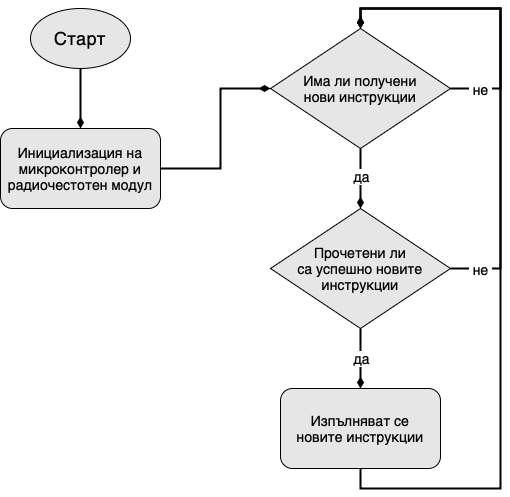
\includegraphics[width=0.6\linewidth]{images/logic-schema-robot.png}
    
    \caption{Логическа схема на робота}
    \label{fig:logic-robot} 
\end{figure}


%================================================================================
% СОФТУЕР  -  РАДИО

\section{Софтуерна реализация на библиотеката на радиочестотния модул}
\label{sec:library}

Безжичната комуникация между дистанционното и бойния робот се осъществава посредством радиочестотния модул nRF24L01 на компанията Nordic. За целите на дипломния проект не беше употребявана готова библиотека за управление на избрания модул, а беше разработена собствена такава. За нейната реализация са употребявани функционалностите на вградената HAL библиотека. С цел улеснение на написването на библиотеката, в заглавния файл са дефинирани като макроси адресите в паметта на регистрите и SPI командните думи. За да може библиотеката да работи, предварително трябва да бъде конфигуриран SPI интерфейса и пиновете, които се използват nRF модула. С цел улеснение на работата с библиотеката е предвидено предварително изводите на радиочестотния модул да имат зададени потребителските етикети NRF24L01\_CSN, NRF24L01\_CE и NRF24L01\_IRQ на съответните им пинове на микроконтролера.

Основните функционалности, които трябва да бъдат реализирани, за да може библиотеката да бъде разработена са писане и четене на регистрите на радиочестотния модул. За да се пише в регистър се подготвя масив с дължина 2 байта. В първия се поставя номера на регистъра, а във втория стойността, която трябва да бъде записана. За да може nRF модула да разбере, че трябва да запише получената стойност, трябва да бъде поставена единица на 5-та позиция от първия байт. Съгласно секция 8.3. "SPI комуникация" от документацията на nRF24L01 всяка SPI операция трябва да бъде започната с падащ фронт на CSN извода на радиочестотния модул. След това се извиква HAL функцията за предаване на информация по SPI интерфейса.

\lstinputlisting[language=c, consecutivenumbers=false, linerange={37-51}, caption={Писане в регистър}, label={lst:write-register}]{documents/rf-library/NRF24L01.c}

Четенето на регистър се реализира аналогично. При него не се подготвя масив, в който да се постави адреса на регистъра и той не бива редактиран. Вместо това първо се използва HAL функцията за предаване на номера на регистъра, който трябва да бъде прочетен, и след това се използва HAL функцията за получаване на данни по SPI.

\lstinputlisting[language=c, consecutivenumbers=false, linerange={72-87}, caption={Четене на регистър}, label={lst:read-register}]{documents/rf-library/NRF24L01.c}

Основната част от регистрите в паметта на използвания nRF модул са с размер 1 байт, но тези, които съхраняват адреси за каналите за комуникация 0 и 1 имат 5 пъти по-голяма дължина. Поради тази причина са написани функциите nrf24\_write\_reg\_multi() и nrf24\_read\_reg\_multi(), които съответно могат да бъдат видени на \autoref{lst:write-big-register} и \autoref{lst:read-big-register}. Те са реализирани аналогично на по-малките им подобни функции.

\lstinputlisting[language=c, consecutivenumbers=false, linerange={52-70}, caption={Писане на големи регистри}, label={lst:write-big-register}]{documents/rf-library/NRF24L01.c}

\lstinputlisting[language=c, consecutivenumbers=false, linerange={88-99}, caption={Четене на големи регистри}, label={lst:read-big-register}]{documents/rf-library/NRF24L01.c}


%================================================================================
% ИНИЦИАЛИЗАЦИЯ

\subsection{Инициализация на модула}
\label{ssec:init}

При получаване на захранване първата задача на микроконтролера и радио модула е да бъдат конфигурирани. Инициализацията на първия може да бъде видяна в \cref{ssec:init-controller} и \cref{ssec:init-robot}. Привеждането на радиочестотния модул в състояние, което позволява безжично предаване на информация е осъществено като се извикват една след друга първо функцията за инициализация на модула и след това и допълнителна такава, с която се пояснява дали същия е предавател или получател на информацията.

При началото на инициализацията на CE пина се подава ниско ниво за да се гарантира, че няма да се активира механизма за изпращане на данни. След това се подават зануляват стойностите на CONFIG и RF\_CH регистрите. Те следва да бъдат редактирани при задаването на роля на модула(предавател или приемник). Чрез записване на 0 в EN\_AA регистъра се изключват автоматичните потвърждения по време на безжичното предаване. В регистъра EN\_RXADDR стойността 0 спира употребата на 6-те информационни канала. За да се дефинира дължината на адреса да бъде 5 байта в регистъра SETUP\_AW са поставени единици на битове 0 и 1. Последния регистър, който се конфигурира в рамките на тази функция е RF\_SETUP. Чрез поставяне на 0 на 3 бит в него се задава скоростта на предаване на информация да бъде 1Mbps, а посредством единици на битове 1 и 2, мощността на предаване на изхода на радиото е 0dBm. 

\lstinputlisting[language=c, consecutivenumbers=false, linerange={145-159}, caption={Инициализация на радио модула}, label={lst:init}]{documents/rf-library/NRF24L01.c}

След функцията за инициализиране на nRF модула се извиква функция, която да пояснява дали модула е предавател или получател на данни. В \autoref{lst:conf-transmitter} може да бъде видяна процедурата за конфигуриране предавател. Първо се задава в регистър RF\_CH честотата (канала), на която ще се предава информацията. След това се записва 5 байтовия адрес на получателя в TX\_ADDR регистъра. После без да се редактира останалата част от регистъра в CONFIG се поставят единица на бит 1 и се оставя нула на бит 0 съответно за да се стартира дейността на радиочестотния модул и за да се влезе в режим на изпращач на информация. 

\lstinputlisting[language=c, consecutivenumbers=false, linerange={164-174}, caption={Конфигуриране на изпращач на данни}, label={lst:conf-transmitter}]{documents/rf-library/NRF24L01.c}

Подобно на последно разглежданата функция NRF24\_RX\_mode() започва със задаване на честотата на предаване на информация. След това без да се редактира останалата част от регистъра EN\_RXADDR се поставя единица на бит 1 поради за да се позволи употребата на информационен канал 1. После се записва 5 байтовия адрес на изпращача на информация в RX\_ADDR\_P1 регистъра. За да се дефинира дължината на пакета данни, който ще се изпраща безжично, се записва големината на структурата Payload в регистъра RX\_PW\_P1. След това без да се реактира останалата му част в CONFIG регистъра се поставят единици на битове 0 и 1 съответно за да се стартира дейността на радиочестотния модул и за да се влезе в режим на получател на данни. В края на тази функция CE пина бива поставен във високо състояние и се държи в това през целия период на работа. В случай, че CE мине в ниско ниво, nRF модула ще излезе от режима на получател.

\lstinputlisting[language=c, consecutivenumbers=false, linerange={234-256}, caption={Конфигуриране на получател на данни}, label={lst:conf-receiver}]{documents/rf-library/NRF24L01.c}

Стойностите, които са избрани за скорост на безжичното предаване, мощността на предаване на изхода на nRF модула и честотата на излъчване на сигнали са подбрани такива, че да осигуряват максимален обхват на безжичната комуникация.

%================================================================================
% ИЗПРАЩАНЕ НА ДАННИ

\subsection{Изпращане на информация}
\label{ssec:transmit}

Изпращането на пакет инструкции от дистанционното към робота се извършва посредством функцията NRF24\_transmit(). Първата стъпка от нейното изпълнение е пакета с инструкции да бъде зареден в паметта на радио модула, посредством функцията, която може да бъде видяна в \autoref{lst:push-payload}. След това се генерира импулс на CE извода по-дълъг от 10us. Съгласно секция 6.1.5. "режим предаване" от документацията на nRF24L01 при такъв импулс в режима за изпращане на данни, записаните в паметта на модула пакети инструкции започват да се излъчват. Останалата част на функцията проверява дали пакетите са били изпратени успешно като проверява съдържанието на FIFO\_STATUS регистъра. Ако четвъртият бит в него е вдигнат означава, че пакета е бил успешно изпратен.

\lstinputlisting[language=c, consecutivenumbers=false, linerange={204-228}, caption={Изпращане на пакет инструкции}, label={lst:transmit}]{documents/rf-library/NRF24L01.c}

Когато се зарежда пакет инструкции в паметта на радиочестотния модул, първо се проверява дали пакета не е твърде голям. В случай, че е опита за безжично изпращане на инструкциите бива прекратен. Останалата част от зареждането на пакета наподобява значително функциите за писане в регистри. Първо се заделя масив от еднобайтови променливи. След това на първа позиция в масива се записва SPI командата за записване на пакета в паметта на модула и чрез функцията memcpy() се записва съдържанието на пакета в масива от втория елемент нататък. Както беше споменато в предишната секция следва да се направи падащ фронт на пин CSN. Когато буфера е вече готов, той бива зареден в паметта, чрез HAL функцията за предаване на информация по SPI интерфейса. Накрая функцията завършва като CSN пина ве върне в свойто предишно състояние.

\lstinputlisting[language=c, consecutivenumbers=false, linerange={175-202}, caption={Зареждане на пакет инструкции}, label={lst:push-payload}]{documents/rf-library/NRF24L01.c}

%================================================================================
% ПОЛУЧАВАНЕ НА ДАННИ

\subsection{Получаване на информация}
\label{ssec:receive}

Получаването на пакети с инструкции се реализира чрез две функции. Първата проверява дали има нова получена информация в радио модула, а втората е същинското и извличане в паметта на микроконтролера. Проверката се осъществява като се прочита STATUS регистъра. Ако бит 6 е единица следва, че има получени нови команди, а в битове 1, 2 и 3 е запазен номера на информационния канал, от който е получената информация. След това стойността на същия регистър се рестартира и функцията връща резултат, показващ, че има получени данни. 

\lstinputlisting[language=c, consecutivenumbers=false, linerange={256-273}, caption={Проверка дали има получен пакет инструкции}, label={lst:check-delivered}]{documents/rf-library/NRF24L01.c}

Във функцията за извличане на данни първата първо се дефинират двата помощни масива. В първия се записва SPI командата R\_RX\_PAYLOAD, която се използва за да се извлече получения нов пакет информация, а във втория следва тя да се бъде записана. След това посредством HAL функцията за предаване и получаване на информация по SPI интерфейса командата се изпраща до радиочестотния модул и сеполучава резултата във втория помощен масив. После чрез функцията memcpy() информацията се премества от помощния регистър в желаната променлива.

\lstinputlisting[language=c, consecutivenumbers=false, linerange={275-299}, caption={Получаване на пакет инструкции}, label={lst:receive}]{documents/rf-library/NRF24L01.c}



%================================================================================
% СОФТУЕР  -  ДИСТАНЦИОННО

\section{Софтуерна реализация на дистанционното}
\label{sec:software-controller}

Както e описано в \cref{sec:block-schemas} компонентите, които се използват в дистанционното са 2 потенциометъра и 3 бутона.

%================================================================================
% ИНИЦИАЛИЗАЦИЯ

\subsection{Инициализация на микроконтролера на дистанционното}
\label{ssec:init-controller}

След като получи захранването си микроконтролера преминава през серия от процеси, които трябва да конфигурират използваните периферии, изводи и променливи. Посредством функцията HAL\_Init() се рестартират всички периферии и се инициализират HAL библиотеката и всички нейни функционалности. След това чрез SystemClock\_Config() се конфигурира системния таймер. После следва конфигурацията на изводите на микроконтролера. Една от тях може да бъде видяна в \autoref{lst:conf-pin-controller}. За това кой пин как е конфигуриран и за какво се използва може да се разбере от таблица \cref{table:pins-controller}. След това се инициализира SPI връзката с nRF модула. Чрез MX\_TIM4\_Init() се инициализира таймер 4, с помощта на когото се изпращат пакетите с инструкции на равни периоди. След това се инициализират и двата аналогово-цифрови преобразувателя, които се използват за четене на състоянието на потенциометрите. Последната инициализация е тази на радиочестотния модул и се задава неговия режим на работа. Преди да започне повтарящият се цикъл на работа таймера се стартира и се пуска калибрация на аналогово-цифровите преобразуватели.

\lstinputlisting[language=c, consecutivenumbers=false, linerange={72-76}, caption={Конфигуриране на пин}, label={lst:conf-pin-controller}]{documents/controller/gpio.c}

\begin{table}[H]
    \centering
    \begin{tabular}{| m{4cm} | m{3,5cm} | m{3,5cm} | m{3,5cm} |}
        \hline
        & Wi-fi & Bluetooth & nRF24L01+ \\
        \hline
        Скорост &  Висока & Средно & Средна \\
        \hline
        Обхват & 10ки метри & 10 метра & 10-150 метра \\
        \hline
        Енергийна консумация & Висока & Средна & Ниска\\
        \hline
    \end{tabular}
    \caption{Пинове}
    \label{table:pins-controller}
\end{table}

%================================================================================
% РАБОТЕН ЦИКЪЛ

\subsection{Работен цикъл на дистанционното}
\label{ssec:loop-controller}

Както е описано в \cref{sec:logic-schemas} цикъла на работа се повтаря на равни интервали. Това е постигнато посредством прекъсването при преливане на таймер 4. Той е конфигуриран така, че прекъсването да бъде генерирано на всяка десета от секундата. След извикването на прекъсването се вдига флага send\_flag. При това действие се прочитат състоянията на потенциометрите и се записват на полетата за скорост на лявото и дясното колело. Това е последвано от извикването на функцията за калибриране на данните. В края на този цикъл се инициира изпращане на пакета с инструкциите и при успех се сменя състоянието на вградения светодиод.

\lstinputlisting[language=c, consecutivenumbers=false, linerange={113-134}, caption={Работен цикъл}, label={lst:loop-controller}]{documents/controller/controller.c}

Успоредно на това има конфигурирани и външни прекъсвания. Те имат функцията да редактират позицията на ръката и да пускат или спират движението на оръжието.




%================================================================================
% СОФТУЕР  -  РОБОТ

\section{Софтуерна реализация на управлението на робота}
\label{sec:software-robot}

%================================================================================
% ИНИЦИАЛИЗАЦИЯ

\subsection{Инициализация на микроконтролера на робота}
\label{ssec:init-robot}

След като получи захранването си микроконтролера преминава през серия от процеси, които трябва да конфигурират използваните периферии, изводи и променливи. Посредством функцията HAL\_Init() се рестартират всички периферии и се инициализират HAL библиотеката и всички нейни функционалности. След това чрез SystemClock\_Config() се конфигурира системния таймер. После следва конфигурацията на изводите на микроконтролера. Една от тях може да бъде видяна в \autoref{lst:conf-pin-robot}. За това кой пин как е конфигуриран и за какво се използва може да се разбере от таблица \cref{table:pins-robot}. След това се инициализира SPI връзката с nRF модула. Чрез функциите MX\_TIM3\_Init(), MX\_TIM2\_Init() и MX\_TIM4\_Init() се инициализират таймери 2, 3 и 4. Таймер 3 се използва за генериране широчинно импулсен сигнал за контролиране на скоростта на въртене на четковите мотори, а 4-тия се използва за измерване на тяхната скорост. Таймер 2 се използва за генерирането на импулси за движението на робота. След това се инициализира радиочестотния модул и се задава неговия режим на робота. Чрез функцията HAL\_TIM\_PWM\_Start() се стартира генерирането на широчинно импулсния сигнал. Преди да започне повтарящият се цикъл на работа и таймери 2 и 4 се стартират.

\lstinputlisting[language=c, consecutivenumbers=false, linerange={72-76}, caption={Конфигуриране на пин}, label={lst:conf-pin-robot}]{documents/controller/gpio.c}

\begin{table}[H]
    \centering
    \begin{tabular}{| m{4cm} | m{3,5cm} | m{3,5cm} | m{3,5cm} |}
        \hline
        & Wi-fi & Bluetooth & nRF24L01+ \\
        \hline
        Скорост &  Висока & Средно & Средна \\
        \hline
        Обхват & 10ки метри & 10 метра & 10-150 метра \\
        \hline
        Енергийна консумация & Висока & Средна & Ниска\\
        \hline
    \end{tabular}
    \caption{Пинове}
    \label{table:pins-robot}
\end{table}

%================================================================================
% РАБОТЕН ЦИКЪЛ

\subsection{Работен цикъл на робота}
\label{ssec:loop-robot}

Както е описано в \cref{sec:logic-schemas} цикъла на работа започва с проверка на това дали има получен нов пакет инструкции. Ако има получен такъв се извиква функцията за извличане на данните от радиочестотния модул и ако е успешна се извиква функцията, която прилага инструкциите.

\lstinputlisting[language=c, consecutivenumbers=false, linerange={122-135}, caption={Работен цикъл}, label={lst:loop-robot}]{documents/robot/robot.c}

Функцията за прилагането на инструкциите е съставена от помощни функции. Първо чрез функцията get\_brushed\_DIR() се проверява в коя посока кой от четковите мотори трябва да се върти и се задава съответната стойност на съответния извод. След това посредством get\_brushed\_DIR() се задава какъв трябва да бъде коефициента на запълване на широчинно-импулсния сигнал, който се използва за дава каква трябва да бъде скоростта на въртене на четковите мотори.

\lstinputlisting[language=c, consecutivenumbers=false, linerange={249-280}, caption={Управление на четковите мотори}, label={lst:dc-motor}]{documents/robot/robot.c}

Последната функция, която се извиква във функцията unload\_payload() се казва get\_hand\_DIR(). Тя се използва за да се определя посоката на движение на стъпковия мотор. Импулсите за колко стъпки да бъдат направени се генерират чрез прекъсването при преливане на таймер 2. Функцията за обработка на прекъсването може да бъде видяна в \cref{lst:overflow-interupts}.

\lstinputlisting[language=c, consecutivenumbers=false, linerange={282-297}, caption={Управление на стъпковия мотор}, label={lst:stepper-motor}]{documents/robot/robot.c}

%================================================================================
% СЕНЗОРИ ЗА ОБРАТНА ВРЪЗКА

\subsection{Сензори за обратна връзка}
\label{ssec:feedback-sensors}

Съгласно изискванията за безопасност описани в \cref{sec:requirements} са имплементирани и двата крайни изключвателя за ръката. Те са свързани към изводи на микроконтролера, за които има конфигурирани външни прекъсвания, които се генерират при падащ и нарастващ фронт на вълната. Когато такова прекъсване се появи се вдига флаг, който спира работата на движението на ръката докато ръката не отвори отново крайния изключвател. 

\lstinputlisting[language=c, consecutivenumbers=false, linerange={184-209}, caption={Външни прекъсвания}, label={lst:external-interupts}]{documents/robot/robot.c}

В проекта има монтирани и оптични сензори, чрез които се следи приблизителната скорост на четковите мотори. Тази функционалност е реализирана посредством външни прекъсвания и прекъсване при преливане. При генерирането на първото се увеличава променлива, която съдържа броя завъртания на съответния мотор. Чрез прекъсването при преливане на таймер 4, на равни интервали от време, се проверява дали има направени завъртания за текущия период. Ако няма направени следва да бъде забранено на съответния мотор да се върти известно време.

\lstinputlisting[language=c, consecutivenumbers=false, linerange={211-247}, caption={Прекъсвания при преливане}, label={lst:overflow-interupts}]{documents/robot/robot.c}


